\documentclass[11pt,a4paper]{article}
\usepackage[utf8]{inputenc}
\usepackage[margin=1in]{geometry}
\usepackage{amsmath,amsfonts,amssymb}
\usepackage{graphicx}
\usepackage{tikz}
\usepackage{pgfgantt}
\usepackage{booktabs}
\usepackage{array}
\usepackage{enumitem}
\usepackage{xcolor}
\usepackage{hyperref}
\usepackage{fancyhdr}
\usepackage{titlesec}

% Colors
\definecolor{gridBlue}{RGB}{41,128,185}
\definecolor{gridLightBlue}{RGB}{52,152,219}
\definecolor{gridGreen}{RGB}{46,204,113}
\definecolor{gridOrange}{RGB}{230,126,34}

% Header and footer
\pagestyle{fancy}
\fancyhf{}
\fancyhead[L]{Grid Maker - Project Document}
\fancyhead[R]{Version 2.0}
\fancyfoot[C]{\thepage}

% Title formatting
\titleformat{\section}{\Large\bfseries\color{gridBlue}}{\thesection}{1em}{}
\titleformat{\subsection}{\large\bfseries\color{gridLightBlue}}{\thesubsection}{1em}{}
\titleformat{\subsubsection}{\normalsize\bfseries\color{gridBlue}}{\thesubsubsection}{1em}{}

% Hyperlink setup
\hypersetup{
    colorlinks=true,
    linkcolor=gridBlue,
    urlcolor=gridOrange,
    citecolor=gridLightBlue
}

\begin{document}

% Title page
\begin{titlepage}
\centering
\vspace*{2cm}

{\Huge\bfseries\color{gridBlue} Grid Maker}\\[0.5cm]
{\Large Project Document}\\[2cm]

\begin{tabular}{ll}
\textbf{Assignment:} & Assignment 2 - Grid Maker \\
\textbf{Start Date:} & September 25, 2025 \\
\textbf{Due Date:} & October 10, 2025, 11:59 PM \\
\textbf{Project Duration:} & 2 weeks (16 days) \\
\textbf{Team Size:} & 2 developers (David \& Kevin) \\
\textbf{Document Version:} & 2.0 \\
\textbf{Last Updated:} & October 9, 2025 \\
\end{tabular}

\vfill

{\large An interactive web application for creating and manipulating dynamic grids with color customization.}

\end{titlepage}

% Table of Contents
\tableofcontents
\newpage

\section{Feature Requirements}

\subsection{Core Features}

\subsubsection{Grid Structure Management}
\begin{itemize}[leftmargin=*]
    \item \textbf{Add Rows}: Users can dynamically add rows to the grid
    \item \textbf{Add Columns}: Users can dynamically add columns to the grid
    \item \textbf{Remove Rows}: Users can remove rows from the existing grid
    \item \textbf{Remove Columns}: Users can remove columns from the existing grid
    \item \textbf{Dynamic Updates}: Grid updates immediately upon user actions
\end{itemize}

\subsubsection{Color Management System}
\begin{itemize}[leftmargin=*]
    \item \textbf{Color Selection}: Dropdown menu with multiple color options
    \item \textbf{Single Cell Coloring}: Click individual cells to apply the selected color
    \item \textbf{Fill Uncolored Cells}: Apply selected color to all uncolored cells at once
    \item \textbf{Fill All Cells}: Apply selected color to all cells regardless of current color
    \item \textbf{Clear Grid}: Reset all cells to their initial color (white)
\end{itemize}

\subsubsection{User Interface Elements}
\begin{itemize}[leftmargin=*]
    \item \textbf{Action Menu}: Dropdown menu for selecting grid operations
    \item \textbf{Color Picker}: Dropdown menu for selecting colors
    \item \textbf{Interactive Grid}: Clickable cells that respond to user interactions
    \item \textbf{Visual Feedback}: Clear indication of selected colors and cell states
\end{itemize}

\subsection{Technical Requirements}

\subsubsection{DOM Manipulation}
\begin{itemize}[leftmargin=*]
    \item Use of \texttt{getElementById()} for element selection
    \item Use of \texttt{getElementsByTagName()} for collection retrieval
    \item Use of \texttt{querySelector()} and \texttt{querySelectorAll()} for advanced selection
    \item Use of \texttt{createElement()} for dynamic element creation
    \item Use of \texttt{appendChild()} and \texttt{removeChild()} for DOM tree manipulation
    \item Use of \texttt{insertCell()}, \texttt{deleteCell()}, \texttt{insertRow()}, \texttt{deleteRow()} for table operations
\end{itemize}

\subsubsection{Event Handling}
\begin{itemize}[leftmargin=*]
    \item \texttt{onchange} events for dropdown menu selections
    \item \texttt{onclick} events for cell interactions
    \item Event listeners for user actions
    \item Dynamic event binding for newly created elements
\end{itemize}

\subsubsection{Node Properties}
\begin{itemize}[leftmargin=*]
    \item Use of \texttt{node.children} for accessing child elements
    \item Use of \texttt{node.lastElementChild} for accessing last child
    \item Traversal of DOM tree structure
\end{itemize}

\subsection{Version Control Requirements}

\subsubsection{Git Workflow}
\begin{itemize}[leftmargin=*]
    \item \textbf{Feature Branches}: Separate branch for each user story
    \item \textbf{Pull Requests}: Merge feature branches via pull requests
    \item \textbf{Commit Practices}: Small, frequent commits with descriptive messages
    \item \textbf{Branch Naming}: Clear, descriptive branch names (e.g., feature/add-rows)
\end{itemize}

\subsection{Deployment Requirements}

\begin{itemize}[leftmargin=*]
    \item Website deployed to GitHub Pages
    \item Live URL accessible and functional
    \item README includes link to deployed site
    \item All features working in production environment
\end{itemize}

\section{Application Architecture Description and Diagram}

\subsection{Architecture Overview}

The Grid Maker application follows a \textbf{client-side web application architecture} using vanilla JavaScript for DOM manipulation. The architecture emphasizes \textbf{event-driven programming} and \textbf{dynamic content generation}.

\subsection{System Components}

\subsubsection{Presentation Layer (HTML)}
\begin{itemize}[leftmargin=*]
    \item \textbf{User Interface}: Action menu, color picker, and grid container
    \item \textbf{Semantic Structure}: Proper HTML5 elements for accessibility
    \item \textbf{Dynamic Grid}: Table element that updates based on user actions
    \item \textbf{Form Controls}: Select elements for user input
\end{itemize}

\subsubsection{Styling Layer (CSS)}
\begin{itemize}[leftmargin=*]
    \item \textbf{Grid Styling}: Visual appearance of grid cells and borders
    \item \textbf{Control Styling}: Professional appearance for menus and buttons
    \item \textbf{Responsive Design}: Adaptable layout for different screen sizes
    \item \textbf{Color Themes}: Consistent color scheme throughout application
    \item \textbf{Hover Effects}: Visual feedback for interactive elements
\end{itemize}

\subsubsection{Application Logic Layer (JavaScript)}
\begin{itemize}[leftmargin=*]
    \item \textbf{Grid Manager}: Functions for adding/removing rows and columns
    \item \textbf{Color Manager}: Functions for applying colors to cells
    \item \textbf{Event Manager}: Handlers for user interactions
    \item \textbf{State Manager}: Tracking current selected action and color
    \item \textbf{Cell Manager}: Individual cell click handlers and color application
\end{itemize}

\subsection{Architecture Diagram}

\begin{figure}[h]
\centering
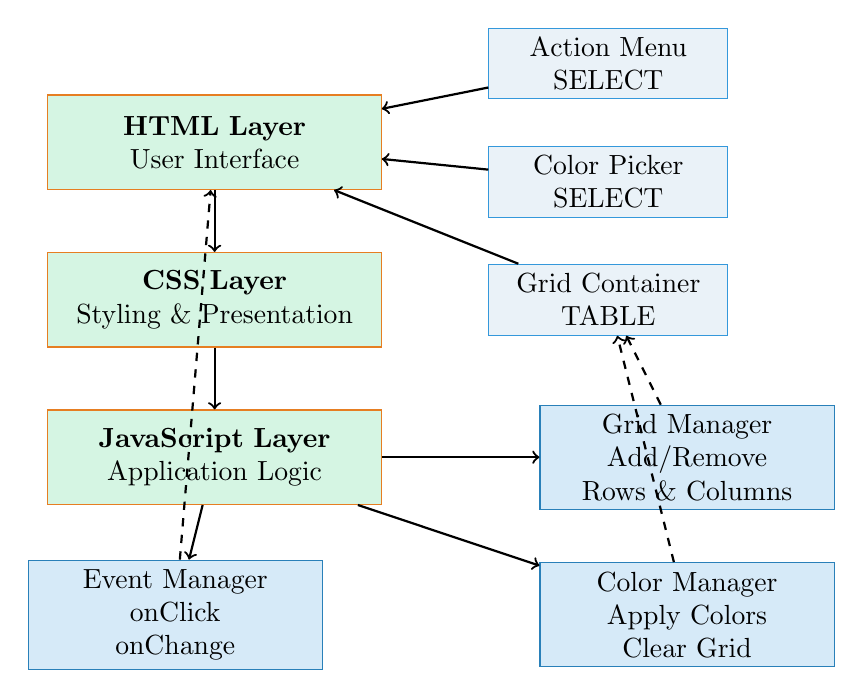
\begin{tikzpicture}[
    box/.style={rectangle, draw=gridBlue, fill=gridLightBlue!20, text width=3.5cm, text centered, minimum height=1cm},
    layer/.style={rectangle, draw=gridOrange, fill=gridGreen!20, text width=4cm, text centered, minimum height=1.2cm},
    small/.style={rectangle, draw=gridLightBlue, fill=gridBlue!10, text width=2.8cm, text centered, minimum height=0.8cm}
]

% Layers
\node[layer] (html) at (0,0) {\textbf{HTML Layer}\\User Interface};
\node[layer] (css) at (0,-2) {\textbf{CSS Layer}\\Styling \& Presentation};
\node[layer] (js) at (0,-4) {\textbf{JavaScript Layer}\\Application Logic};

% HTML Components
\node[small] (menu) at (5,1) {Action Menu\\SELECT};
\node[small] (color) at (5,-0.5) {Color Picker\\SELECT};
\node[small] (grid) at (5,-2) {Grid Container\\TABLE};

% JavaScript Components
\node[box] (gridmgr) at (6,-4) {Grid Manager\\Add/Remove\\Rows \& Columns};
\node[box] (colormgr) at (6,-6) {Color Manager\\Apply Colors\\Clear Grid};
\node[box] (eventmgr) at (-0.5,-6) {Event Manager\\onClick\\onChange};

% Connections
\draw[->, thick] (html) -- (css);
\draw[->, thick] (css) -- (js);
\draw[->, thick] (menu) -- (html);
\draw[->, thick] (color) -- (html);
\draw[->, thick] (grid) -- (html);
\draw[->, thick] (js) -- (gridmgr);
\draw[->, thick] (js) -- (colormgr);
\draw[->, thick] (js) -- (eventmgr);
\draw[->, thick, dashed] (eventmgr) -- (html);
\draw[->, thick, dashed] (gridmgr) -- (grid);
\draw[->, thick, dashed] (colormgr) -- (grid);

\end{tikzpicture}
\caption{Grid Maker Application Architecture}
\end{figure}

\subsection{Data Flow}

\begin{enumerate}[leftmargin=*]
    \item \textbf{User Interaction}: User selects action from menu or color from picker
    \item \textbf{Event Capture}: JavaScript event handlers capture the selection
    \item \textbf{State Update}: Application updates internal state (selected action/color)
    \item \textbf{Action Execution}: Based on selection, appropriate function is called
    \item \textbf{DOM Manipulation}: Functions modify the DOM (add/remove cells, apply colors)
    \item \textbf{Visual Update}: Browser re-renders the updated grid
    \item \textbf{Event Binding}: New elements receive appropriate event listeners
\end{enumerate}

\subsection{Technology Stack}

\begin{itemize}[leftmargin=*]
    \item \textbf{HTML5}: Structure and semantic markup
    \item \textbf{CSS3}: Styling, layout, and visual effects
    \item \textbf{JavaScript (ES6+)}: Application logic and DOM manipulation
    \item \textbf{Git}: Version control and collaboration
    \item \textbf{GitHub}: Repository hosting and collaboration
    \item \textbf{GitHub Pages}: Static website hosting
\end{itemize}

\subsection{Key Design Patterns}

\begin{itemize}[leftmargin=*]
    \item \textbf{Event-Driven Architecture}: User actions trigger event handlers
    \item \textbf{Separation of Concerns}: HTML (structure), CSS (presentation), JavaScript (behavior)
    \item \textbf{Modular Functions}: Each function has a single, well-defined responsibility
    \item \textbf{Progressive Enhancement}: Core functionality works, enhanced with JavaScript
\end{itemize}

\section{Epics, User Stories, and Acceptance Criteria}

\subsection{Epic 1: Grid Structure Management}

\subsubsection{User Story 1.1: Select Action from Menu}
\textbf{As a} user\\
\textbf{I want to} select an action from a dropdown menu\\
\textbf{So that} I can choose what operation to perform on the grid

\textbf{Acceptance Criteria:}
\begin{itemize}[leftmargin=*]
    \item Action menu is visible and accessible
    \item Menu includes all available actions (Add Row, Add Column, Remove Row, Remove Column, Fill Uncolored, Fill All, Clear Grid)
    \item Selected action is stored and used for subsequent operations
    \item Menu has clear, descriptive labels
    \item onChange event properly captures menu selection
\end{itemize}

\subsubsection{User Story 1.2: Add Rows to Grid}
\textbf{As a} user\\
\textbf{I want to} add rows to the grid\\
\textbf{So that} I can increase the vertical size of my grid

\textbf{Acceptance Criteria:}
\begin{itemize}[leftmargin=*]
    \item Selecting "Add Row" action adds a new row to the bottom of the grid
    \item New row contains the same number of cells as existing rows
    \item New cells have default white background color
    \item New cells are clickable and respond to color application
    \item Grid updates immediately without page refresh
    \item Uses \texttt{insertRow()} method
\end{itemize}

\subsubsection{User Story 1.3: Add Columns to Grid}
\textbf{As a} user\\
\textbf{I want to} add columns to the grid\\
\textbf{So that} I can increase the horizontal size of my grid

\textbf{Acceptance Criteria:}
\begin{itemize}[leftmargin=*]
    \item Selecting "Add Column" action adds a new column to the right side of all rows
    \item Each row receives one new cell at the end
    \item New cells have default white background color
    \item New cells are clickable and respond to color application
    \item Grid updates immediately without page refresh
    \item Uses \texttt{insertCell()} method
\end{itemize}

\subsubsection{User Story 1.4: Remove Rows from Grid}
\textbf{As a} user\\
\textbf{I want to} remove rows from the grid\\
\textbf{So that} I can decrease the vertical size of my grid

\textbf{Acceptance Criteria:}
\begin{itemize}[leftmargin=*]
    \item Selecting "Remove Row" action removes the last row from the grid
    \item Grid prevents removal if only one row remains (or implements minimum row logic)
    \item Grid updates immediately without page refresh
    \item No errors occur when attempting to remove from minimum grid
    \item Uses \texttt{deleteRow()} method
\end{itemize}

\subsubsection{User Story 1.5: Remove Columns from Grid}
\textbf{As a} user\\
\textbf{I want to} remove columns from the grid\\
\textbf{So that} I can decrease the horizontal size of my grid

\textbf{Acceptance Criteria:}
\begin{itemize}[leftmargin=*]
    \item Selecting "Remove Column" action removes the last cell from each row
    \item Grid prevents removal if only one column remains (or implements minimum column logic)
    \item Grid updates immediately without page refresh
    \item No errors occur when attempting to remove from minimum grid
    \item Uses \texttt{deleteCell()} method
\end{itemize}

\subsection{Epic 2: Color Management System}

\subsubsection{User Story 2.1: Select Color from Dropdown}
\textbf{As a} user\\
\textbf{I want to} select a color from a dropdown menu\\
\textbf{So that} I can choose which color to apply to grid cells

\textbf{Acceptance Criteria:}
\begin{itemize}[leftmargin=*]
    \item Color picker dropdown is visible and accessible
    \item Menu includes multiple color options (at least 5-7 colors)
    \item Color names are clear and descriptive
    \item Selected color is stored and used for cell coloring
    \item onChange event properly captures color selection
    \item Colors are standard HTML/CSS colors or hex values
\end{itemize}

\subsubsection{User Story 2.2: Color Single Cell}
\textbf{As a} user\\
\textbf{I want to} click on a cell to color it\\
\textbf{So that} I can color individual cells with my selected color

\textbf{Acceptance Criteria:}
\begin{itemize}[leftmargin=*]
    \item Clicking a cell applies the currently selected color to that cell
    \item Cell color updates immediately upon click
    \item Previously colored cells can be recolored
    \item onClick event properly captures cell clicks
    \item Cell background color changes visibly
    \item All cells are individually clickable
\end{itemize}

\subsubsection{User Story 2.3: Color All Uncolored Cells}
\textbf{As a} user\\
\textbf{I want to} fill all uncolored cells with the selected color\\
\textbf{So that} I can quickly color empty cells without clicking each one

\textbf{Acceptance Criteria:}
\begin{itemize}[leftmargin=*]
    \item Action applies selected color only to cells with default/white color
    \item Previously colored cells remain unchanged
    \item All uncolored cells update simultaneously
    \item Action works correctly regardless of grid size
    \item Uses \texttt{querySelectorAll()} or similar to find uncolored cells
\end{itemize}

\subsubsection{User Story 2.4: Color All Cells}
\textbf{As a} user\\
\textbf{I want to} fill all cells with the selected color\\
\textbf{So that} I can change the entire grid to a single color quickly

\textbf{Acceptance Criteria:}
\begin{itemize}[leftmargin=*]
    \item Action applies selected color to every cell in the grid
    \item All cells change color regardless of previous color
    \item All cells update simultaneously
    \item Action works correctly regardless of grid size
    \item Uses \texttt{getElementsByTagName()} or \texttt{querySelectorAll()} to select all cells
\end{itemize}

\subsubsection{User Story 2.5: Clear All Cells}
\textbf{As a} user\\
\textbf{I want to} clear all cell colors\\
\textbf{So that} I can reset the grid to its initial state

\textbf{Acceptance Criteria:}
\begin{itemize}[leftmargin=*]
    \item Action resets all cells to default white color
    \item All cells update simultaneously
    \item Grid structure remains unchanged (rows and columns preserved)
    \item Action works correctly regardless of grid size
    \item Clear action is easily accessible from action menu
\end{itemize}

\subsection{Epic 3: Code Quality and Version Control}

\subsubsection{User Story 3.1: Feature Branch Workflow}
\textbf{As a} developer\\
\textbf{I want to} create feature branches for each user story\\
\textbf{So that} I can develop features in isolation and merge them safely

\textbf{Acceptance Criteria:}
\begin{itemize}[leftmargin=*]
    \item Each user story has its own feature branch
    \item Branch names follow convention (e.g., feature/add-rows, feature/color-cells)
    \item Branches are created from main/master branch
    \item Feature branches are merged via pull requests
    \item Commit history shows clear feature development
\end{itemize}

\subsubsection{User Story 3.2: Clean Code Organization}
\textbf{As a} developer\\
\textbf{I want to} maintain clean, well-organized code\\
\textbf{So that} the code is easy to read, understand, and maintain

\textbf{Acceptance Criteria:}
\begin{itemize}[leftmargin=*]
    \item Code is properly indented and formatted
    \item Functions have descriptive names
    \item Variables have meaningful names
    \item Comments explain complex logic
    \item Code follows consistent style guidelines
    \item Separate files for HTML, CSS, and JavaScript
\end{itemize}

\subsection{Epic 4: Deployment and Documentation}

\subsubsection{User Story 4.1: GitHub Pages Deployment}
\textbf{As a} user\\
\textbf{I want to} access the Grid Maker online\\
\textbf{So that} I can use it without downloading files

\textbf{Acceptance Criteria:}
\begin{itemize}[leftmargin=*]
    \item Website is deployed to GitHub Pages
    \item Live URL is accessible and functional
    \item All features work in production environment
    \item README includes link to live site
    \item No console errors in production
\end{itemize}

\subsubsection{User Story 4.2: Project Documentation}
\textbf{As a} team member or external developer\\
\textbf{I want to} read clear documentation\\
\textbf{So that} I understand the project structure and how to contribute

\textbf{Acceptance Criteria:}
\begin{itemize}[leftmargin=*]
    \item README includes project description
    \item README lists group member names and GitHub usernames
    \item README includes link to GitHub Pages deployment
    \item README explains how to run the project locally
    \item Project document (PDF) includes all required sections
\end{itemize}

\section{Project Schedule Chart (Gantt Chart)}

\subsection{Project Timeline Overview}

\textbf{Project Duration}: 2 weeks (16 days)\\
\textbf{Start Date}: September 25, 2025\\
\textbf{Due Date}: October 10, 2025, 11:59 PM\\
\textbf{Team Size}: 1-4 developers

\subsection{Detailed Gantt Chart}

\begin{figure}[h]
\centering
\begin{ganttchart}[
    x unit=0.7cm,
    y unit title=0.6cm,
    y unit chart=0.5cm,
    vgrid,
    hgrid,
    title label font=\bfseries\footnotesize,
    bar label font=\footnotesize,
    group label font=\small,
    milestone label font=\footnotesize,
    bar/.append style={fill=gridLightBlue!80},
    milestone/.append style={fill=gridOrange,rounded corners=2pt},
    group/.append style={fill=gridBlue!60}
]{1}{16}

\gantttitle{Grid Maker Project Timeline}{16} \\
\gantttitle{September}{6}
\gantttitle{October}{10} \\
\gantttitlelist{25,26,27,28,29,30,1,2,3,4,5,6,7,8,9,10}{1} \\

\ganttgroup{Planning \& Setup}{1}{3} \\
\ganttbar{Project Planning}{1}{2} \\
\ganttbar{Repository Setup}{1}{2} \\
\ganttbar{Initial HTML/CSS}{2}{3} \\
\ganttbar{Project Document Draft}{2}{3} \\

\ganttgroup{Grid Structure (Stories 1-5)}{3}{9} \\
\ganttbar{US 1: Action Menu}{3}{4} \\
\ganttbar{US 2: Add Rows}{4}{5} \\
\ganttbar{US 3: Add Columns}{5}{6} \\
\ganttbar{US 4: Remove Rows}{6}{7} \\
\ganttbar{US 5: Remove Columns}{7}{9} \\

\ganttgroup{Color Management (Stories 6-10)}{9}{13} \\
\ganttbar{US 6: Color Picker}{9}{10} \\
\ganttbar{US 7: Color Single Cell}{10}{11} \\
\ganttbar{US 8: Color Uncolored}{11}{12} \\
\ganttbar{US 9: Color All Cells}{12}{13} \\
\ganttbar{US 10: Clear Grid}{12}{13} \\

\ganttgroup{Testing \& Deployment}{13}{16} \\
\ganttbar{Testing \& Bug Fixes}{13}{15} \\
\ganttbar{Code Review \& Cleanup}{14}{15} \\
\ganttbar{Final Documentation}{15}{16} \\
\ganttbar{GitHub Pages Deploy}{15}{16} \\
\ganttbar{PDF \& Submission Prep}{16}{16} \\

\ganttmilestone{Setup Complete}{3} \\
\ganttmilestone{Grid Features Done}{9} \\
\ganttmilestone{All Features Complete}{13} \\
\ganttmilestone{Project Due}{16}

\end{ganttchart}
\caption{Project Timeline - Gantt Chart (Sept 25 - Oct 10, 2025)}
\end{figure}

\subsection{Phase Breakdown}

\subsubsection{Phase 1: Planning \& Setup (Days 1-3, Sept 25-27)}
\textbf{Tasks:}
\begin{itemize}[leftmargin=*]
    \item Analyze project requirements
    \item Create project document structure
    \item Set up GitHub repository
    \item Create initial HTML structure with basic grid
    \item Set up CSS framework for styling
    \item Initialize JavaScript file
    \item Draft initial project documentation
\end{itemize}

\textbf{Deliverables:}
\begin{itemize}[leftmargin=*]
    \item Project document (initial draft)
    \item GitHub repository with README
    \item Basic HTML/CSS/JS file structure
    \item Initial grid display
\end{itemize}

\textbf{Branch:} \texttt{main/master} (initial setup)

\subsubsection{Phase 2: Grid Structure Management (Days 3-9, Sept 27-Oct 3)}
\textbf{Tasks:}
\begin{itemize}[leftmargin=*]
    \item Implement action menu dropdown
    \item Create add row functionality (feature/add-rows)
    \item Create add column functionality (feature/add-columns)
    \item Create remove row functionality (feature/remove-rows)
    \item Create remove column functionality (feature/remove-columns)
    \item Test grid manipulation across different sizes
\end{itemize}

\textbf{Deliverables:}
\begin{itemize}[leftmargin=*]
    \item Working action menu
    \item Complete row/column add/remove functionality
    \item 5 feature branches with pull requests
    \item Functional grid structure management
\end{itemize}

\textbf{Branches:}
\begin{itemize}[leftmargin=*]
    \item \texttt{feature/action-menu}
    \item \texttt{feature/add-rows}
    \item \texttt{feature/add-columns}
    \item \texttt{feature/remove-rows}
    \item \texttt{feature/remove-columns}
\end{itemize}

\subsubsection{Phase 3: Color Management System (Days 9-13, Oct 3-7)}
\textbf{Tasks:}
\begin{itemize}[leftmargin=*]
    \item Implement color picker dropdown
    \item Create single cell coloring functionality (feature/color-cell)
    \item Create fill uncolored cells functionality (feature/fill-uncolored)
    \item Create fill all cells functionality (feature/fill-all)
    \item Create clear grid functionality (feature/clear-grid)
    \item Test color application and clearing
\end{itemize}

\textbf{Deliverables:}
\begin{itemize}[leftmargin=*]
    \item Working color picker
    \item Complete color management system
    \item 5 feature branches with pull requests
    \item Fully functional grid coloring
\end{itemize}

\textbf{Branches:}
\begin{itemize}[leftmargin=*]
    \item \texttt{feature/color-picker}
    \item \texttt{feature/color-cell}
    \item \texttt{feature/fill-uncolored}
    \item \texttt{feature/fill-all}
    \item \texttt{feature/clear-grid}
\end{itemize}

\subsubsection{Phase 4: Testing, Documentation \& Deployment (Days 13-16, Oct 7-10)}
\textbf{Tasks:}
\begin{itemize}[leftmargin=*]
    \item Comprehensive testing of all features
    \item Cross-browser testing
    \item Code cleanup and refactoring
    \item Add code comments
    \item Complete project document
    \item Update README with team info and deployment link
    \item Deploy to GitHub Pages
    \item Final testing of deployed site
    \item Prepare submission materials (PDF conversion)
\end{itemize}

\textbf{Deliverables:}
\begin{itemize}[leftmargin=*]
    \item Fully tested application
    \item Clean, commented code
    \item Complete project document (PDF)
    \item Updated README
    \item Live website on GitHub Pages
    \item Submission ready for Brightspace
\end{itemize}

\subsection{Milestones}

\begin{itemize}[leftmargin=*]
    \item \textbf{September 27}: Project setup and initial structure complete
    \item \textbf{October 3}: Core grid structure management complete
    \item \textbf{October 7}: All color management features complete
    \item \textbf{October 10}: Project deployed, tested, and submitted
\end{itemize}

\subsection{Risk Management}

\subsubsection{Identified Risks}
\begin{itemize}[leftmargin=*]
    \item \textbf{DOM Manipulation Complexity}: Table manipulation may have edge cases
    \item \textbf{Event Handler Issues}: Dynamically created cells need proper event binding
    \item \textbf{Browser Compatibility}: Different browsers may handle events differently
    \item \textbf{Merge Conflicts}: Multiple feature branches may conflict
    \item \textbf{Time Constraints}: One week is a tight timeline
\end{itemize}

\subsubsection{Mitigation Strategies}
\begin{itemize}[leftmargin=*]
    \item \textbf{Incremental Testing}: Test each feature thoroughly before moving to next
    \item \textbf{Event Delegation}: Use event delegation for dynamically created cells
    \item \textbf{Browser Testing}: Test in Chrome, Firefox, and Edge during development
    \item \textbf{Small Commits}: Make frequent, small commits to minimize conflicts
    \item \textbf{Early Start}: Begin project as soon as assigned
    \item \textbf{Code Reviews}: Review pull requests carefully before merging
\end{itemize}

\subsection{Resource Allocation}

\subsubsection{Team Structure (2-week timeline)}
\begin{itemize}[leftmargin=*]
    \item \textbf{Solo Developer}: All tasks (estimated 20-25 hours over 2 weeks)
    \item \textbf{2-Person Team}: Split features evenly (12-15 hours each over 2 weeks)
    \item \textbf{3-4 Person Team}: Divide by epics (10-12 hours each over 2 weeks)
\end{itemize}

\subsubsection{Recommended Task Division (4-Person Team)}
\begin{itemize}[leftmargin=*]
    \item \textbf{Developer 1}: Project setup, planning, add/remove rows features
    \item \textbf{Developer 2}: Action menu, add/remove columns features
    \item \textbf{Developer 3}: Color picker, single cell coloring, fill operations
    \item \textbf{Developer 4}: Clear grid, testing, documentation, deployment
\end{itemize}

\subsubsection{Required Tools}
\begin{itemize}[leftmargin=*]
    \item \textbf{Text Editor/IDE}: VS Code, Sublime Text, or similar
    \item \textbf{Web Browser}: Chrome, Firefox, or Edge with DevTools
    \item \textbf{Git}: For version control
    \item \textbf{GitHub Account}: For repository hosting and Pages
    \item \textbf{LaTeX Editor}: For project document (Overleaf, TeXShop, etc.)
\end{itemize}

\section{Implementation Notes}

\subsection{Recommended JavaScript Methods}

\subsubsection{Element Selection}
\begin{itemize}[leftmargin=*]
    \item \texttt{document.getElementById('gridTable')} - Get grid table element
    \item \texttt{document.getElementsByTagName('td')} - Get all cells
    \item \texttt{document.querySelector('\#actionMenu')} - Get dropdown menus
    \item \texttt{document.querySelectorAll('td')} - Get all cells with selector
\end{itemize}

\subsubsection{DOM Manipulation}
\begin{itemize}[leftmargin=*]
    \item \texttt{table.insertRow()} or \texttt{table.insertRow(-1)} - Add row at end
    \item \texttt{table.deleteRow(-1)} - Remove last row
    \item \texttt{row.insertCell()} or \texttt{row.insertCell(-1)} - Add cell at end
    \item \texttt{row.deleteCell(-1)} - Remove last cell
    \item \texttt{document.createElement('td')} - Create new cell element
    \item \texttt{element.appendChild(child)} - Add child to element
    \item \texttt{element.removeChild(child)} - Remove child from element
\end{itemize}

\subsubsection{Node Properties}
\begin{itemize}[leftmargin=*]
    \item \texttt{table.children} or \texttt{table.rows} - Access rows
    \item \texttt{row.children} or \texttt{row.cells} - Access cells in row
    \item \texttt{table.lastElementChild} - Get last row
    \item \texttt{row.lastElementChild} - Get last cell in row
\end{itemize}

\subsubsection{Event Handling}
\begin{itemize}[leftmargin=*]
    \item \texttt{element.onchange = function()\{...\}} - Handle dropdown changes
    \item \texttt{element.onclick = function()\{...\}} - Handle click events
    \item \texttt{element.addEventListener('click', handler)} - Add event listener
    \item \texttt{event.target} - Get element that triggered event
\end{itemize}

\subsection{Color Suggestions}

Recommended colors for the color picker:
\begin{itemize}[leftmargin=*]
    \item White (\texttt{\#FFFFFF}) - Default/reset color
    \item Red (\texttt{\#FF0000} or \texttt{red})
    \item Blue (\texttt{\#0000FF} or \texttt{blue})
    \item Green (\texttt{\#00FF00} or \texttt{green})
    \item Yellow (\texttt{\#FFFF00} or \texttt{yellow})
    \item Orange (\texttt{\#FFA500} or \texttt{orange})
    \item Purple (\texttt{\#800080} or \texttt{purple})
    \item Pink (\texttt{\#FFC0CB} or \texttt{pink})
\end{itemize}

\subsection{Best Practices}

\begin{itemize}[leftmargin=*]
    \item \textbf{Start Simple}: Begin with basic grid (e.g., 3x3) and build from there
    \item \textbf{Test Frequently}: Test each feature immediately after implementation
    \item \textbf{Use Console.log}: Debug issues by logging values to console
    \item \textbf{Event Delegation}: Consider using event delegation for cell clicks
    \item \textbf{Validate Input}: Check that rows/columns exist before removing
    \item \textbf{Consistent Naming}: Use clear, consistent variable and function names
    \item \textbf{Comment Complex Logic}: Explain non-obvious code sections
    \item \textbf{Commit Often}: Make small, frequent commits with clear messages
\end{itemize}

\end{document}
